\documentclass[11pt,a4paper]{article}
\usepackage[T1]{fontenc}
\usepackage[utf8]{inputenc}
\usepackage{lmodern}
\usepackage[margin=2.2cm]{geometry}
\usepackage{booktabs,tabularx,array,longtable}
\usepackage{siunitx}
\usepackage{xcolor}
\usepackage{tikz}
\usetikzlibrary{arrows.meta,positioning,fit,calc}
\usepackage{pgfplots}
\pgfplotsset{compat=1.18}
\usepgfplotslibrary{fillbetween}
\usepackage{listings}
\usepackage{enumitem}
\usepackage{caption}
\usepackage{float}
\usepackage[hidelinks,pdfauthor={Yuechao Liu},pdftitle={Internal Display (eDP) Link Failure After Screen Panel Replacement}]{hyperref}

\definecolor{codebg}{HTML}{F5F5F2}
\definecolor{bad}{HTML}{C0392B}
\definecolor{good}{HTML}{1E8449}
\definecolor{phaseA}{HTML}{EEF3F8}
\definecolor{phaseB}{HTML}{E3ECF5}
\definecolor{phaseBB}{HTML}{F9E0DC}
\definecolor{phaseD}{HTML}{E2F1E1}

\lstset{
  basicstyle=\ttfamily\footnotesize,
  backgroundcolor=\color{codebg},
  frame=single, rulecolor=\color{black!15},
  breaklines=true, columns=fullflexible, keepspaces=true,
  showstringspaces=false, upquote=true,
  literate={—}{{---}}1 {°}{{\textdegree}}1 {→}{{$\to$}}1 {…}{{\ldots}}1
}
\newcommand{\reg}[1]{\texttt{#1}}
\setlist{itemsep=2pt,topsep=4pt}
\setlength{\emergencystretch}{3em}
\newcolumntype{Y}{>{\raggedright\arraybackslash}X}

\title{\textbf{Internal Display (eDP) Link Failure After Screen Panel Replacement}\\[4pt]
\large Investigation and Test Report}
\author{Yuechao Liu\\ \href{mailto:yuechao.liu29@gmail.com}{\texttt{yuechao.liu29@gmail.com}}\\[6pt] \small Prepared for the repair service}
\date{23 November 2026}

\begin{document}
\maketitle

\begin{abstract}
\noindent Since the laptop's screen panel was replaced by the official service, the internal display shows
\textbf{thin lines and brief blackouts} that recover by themselves. Using the Linux kernel's DisplayPort debug
logging, we recorded the panel's own link-status registers. They show that the \textbf{embedded DisplayPort (eDP) link between
the mainboard and the panel loses signal lock on all four lanes}, and on one occasion on a single lane only. This happens at \textbf{240\,Hz under
sustained combined CPU+RAM and GPU load}. In a controlled session, idle operation, GPU-only load (12 minutes) and the
\textbf{same combined load at 60\,Hz} produced \textbf{no} link failures and no visible artifacts. The laptop was on AC power with stable voltage throughout. At 240\,Hz the link runs at
8.1\,Gbit/s per lane (the panel's maximum). At 60\,Hz it runs at 4.32\,Gbit/s. The findings point to a marginal physical
connection (eDP cable or connectors, or the replacement panel) that fails when signal margin is lowest. Section~\ref{sec:repro} gives a
step-by-step procedure to reproduce the fault. A test user account running \textbf{GNOME}, with the test cases in its home folder, will be provided
(Section~\ref{sec:testenv}). If you have any questions reproducing or other theories on this issue, feel free to contact me at \href{mailto:yuechao.liu29@gmail.com}{yuechao.liu29@gmail.com}.
\end{abstract}

\tableofcontents
\newpage

%=====================================================================
\section{Result at a glance}
%=====================================================================
\begin{table}[H]
\centering
\caption{Controlled recording session, 23 Nov 2026, 20:43--21:35 (AC power, battery 80\,\%). A link-loss read is a panel status read
in which the lanes were not all locked. Expected link training caused by deliberate refresh-rate switches is excluded.}
\label{tab:phases}
\small
\begin{tabularx}{\linewidth}{@{}c c c Y c c >{\raggedright\arraybackslash}p{2.3cm}@{}}
\toprule
Phase & Time & Refresh & Load & CPU max & Link-loss reads & Visible flicker\\
\midrule
A & 20:48--20:55 & 240\,Hz & none (idle) & \SI{71}{\celsius} & \textcolor{good}{0} & no\\
B & 20:55--21:07 & 240\,Hz & GPU only: OCCT 3D Adaptive + VRAM ($\approx$\SI{88}{W}) & \SI{77}{\celsius} & \textcolor{good}{0} & no\\
B2 & 21:07--21:21 & 240\,Hz & \textbf{GPU + CPU/RAM}: OCCT 3D + VRAM + CPU+RAM & \SI{80}{\celsius} & \textcolor{bad}{\textbf{26} (6 episodes)} & \textbf{yes}, 21:08:41--21:21:13\\
C & 21:21--21:24 & 240\,Hz & none (cool-down) & \SI{77}{\celsius} & \textcolor{good}{0} & ended 21:21:13\\
D & 21:25--21:35 & \textbf{60\,Hz} & GPU + CPU/RAM (same as B2) & \SI{79}{\celsius} & \textcolor{good}{0} & no\\
\bottomrule
\end{tabularx}
\end{table}

\begin{figure}[H]
\centering
\begin{tikzpicture}
\begin{axis}[
  width=\linewidth, height=6.2cm,
  xmin=0, xmax=53, ymin=0, ymax=135,
  xlabel={Minutes since recording start (20:43:06)},
  ylabel={\si{\celsius} \ / \ W},
  legend style={at={(0.5,-0.22)},anchor=north,font=\scriptsize,draw=none,legend columns=3,/tikz/every even column/.append style={column sep=10pt}},
  tick label style={font=\scriptsize}, label style={font=\small},
  clip=false,
]
% phase bands
\fill[phaseA]  (axis cs:5.22,0)  rectangle (axis cs:11.85,135);
\fill[phaseB]  (axis cs:11.85,0) rectangle (axis cs:23.75,135);
\fill[phaseBB] (axis cs:23.75,0) rectangle (axis cs:37.65,135);
\fill[phaseD]  (axis cs:41.77,0) rectangle (axis cs:51.93,135);
\node[font=\scriptsize] at (axis cs:8.5,129) {A idle};
\node[font=\scriptsize] at (axis cs:17.8,129) {B GPU only};
\node[font=\scriptsize,text=bad] at (axis cs:30.7,129) {B2 GPU+CPU/RAM};
\node[font=\scriptsize] at (axis cs:39.7,129) {C};
\node[font=\scriptsize,text=good] at (axis cs:46.85,129) {D same, 60\,Hz};
% flicker marked by user
\draw[bad,line width=2.5pt] (axis cs:25.58,22) -- (axis cs:38.12,22);
\node[font=\scriptsize,text=bad,anchor=south] at (axis cs:31.85,24) {flicker seen by user};
\addplot[black!70, thick] table[x=t,y=cpu] {session.dat};
\addlegendentry{CPU package temperature (\si{\celsius})}
\addplot[blue!70, thin] table[x=t,y=gpuw] {session.dat};
\addlegendentry{NVIDIA GPU power (W)}
\addplot[only marks, mark=|, mark size=6pt, bad, thick] table[x=t,y expr=8] {events.dat};
\addlegendentry{eDP link-loss read}
\end{axis}
\end{tikzpicture}
\caption{Clean session timeline. Link-loss events (red ticks) occur only in phase B2. The same load at 60\,Hz (phase D) and GPU-only load
(phase B) are clean, although CPU temperatures are similar.}
\label{fig:timeline}
\end{figure}

%=====================================================================
\section{System under test}
%=====================================================================
\begin{table}[H]
\centering
\begin{tabularx}{\linewidth}{@{}l Y@{}}
\toprule
Laptop & HP, PCI subsystem ID \reg{103c:8d3f}. It has a display multiplexer: the NVIDIA GPU also has an eDP connector (\reg{card0-eDP-2}), which is disconnected\\
Panel (replacement) & CMN (Chimei Innolux) product \reg{0x1652}, 2560$\times$1600, EDID manufacture date week 21 / 2024. Modes offered: \textbf{60.001\,Hz} and \textbf{240\,Hz} only\\
Panel driven by & Intel Raptor Lake-S UHD Graphics (\reg{i915} driver), connector \reg{card1-eDP-1}, 4-lane eDP, DPCD revision 1.4\\
Discrete GPU & NVIDIA GeForce RTX 5070 Max-Q, open kernel module 620.70.06 (render offload only; it does not drive the panel)\\
Operating system (recorded tests) & Fedora 45, Linux 7.3.4-300.fc45, sway 1.12 (wlroots 0.20.2), Mesa 26.2.7\\
Other software tried & Linux distributions \textbf{CachyOS} and \textbf{Fedora Workstation}; desktop environments \textbf{GNOME}, \textbf{Hyprland} and \textbf{sway}\\
Kernel options (GRUB) & \reg{i915.enable\_psr=0} (Panel Self Refresh disabled for all experiments), nouveau blacklisted\\
Display settings & 2560$\times$1600 at 240\,Hz, scale 1.25, variable refresh rate (adaptive sync) off for all experiments\\
\bottomrule
\end{tabularx}
\end{table}

%=====================================================================
\section{Symptom and history}
%=====================================================================
\begin{itemize}
\item \textbf{Symptom:} thin lines across the screen and occasional blackouts of about one second. The screen recovers by itself. Once
it starts under load, it continues until the load is removed.
\item \textbf{Onset:} after the official service replaced the screen panel. The user ran the same panel model at 240\,Hz before
the repair without this problem.
\item \textbf{User observation before testing:} 60\,Hz does not flicker, 240\,Hz does. Heavy load triggers it.
\item \textbf{Software tried:} the laptop has been run on several Linux distributions (CachyOS, Fedora Workstation) and desktop
environments (GNOME, Hyprland, sway). The problem is not tied to one distribution or desktop environment.
\item \textbf{Conditions under which it appears:} panel at \textbf{240\,Hz}, under sustained \textbf{combined CPU+RAM and GPU load}
(about 2 minutes after the CPU+RAM load is added, in our test). It occurs on AC power. It does \textbf{not} appear at idle, with GPU-only
load, or at \textbf{60\,Hz} under the same load.
\end{itemize}

%=====================================================================
\section{How the data was collected}
\label{sec:methods}
%=====================================================================
All evidence comes from the system's own records: the systemd journal, the kernel log and \reg{/sys}. No third-party
monitoring software was used, apart from OCCT as the load generator.

\paragraph{Test conditions throughout all experiments.} \textbf{Panel Self Refresh (PSR) was disabled} by the kernel argument
\reg{i915.enable\_psr=0}, set in GRUB (\reg{GRUB\_CMDLINE\_LINUX} in \reg{/etc/default/grub}) and confirmed in \reg{/proc/cmdline} at
the start and end of the recorded session. \textbf{Variable refresh rate (adaptive sync) was off} (compositor reports
\reg{adaptive\_sync: disabled}). The panel therefore ran at a fixed refresh rate with a continuously active link, so
the failures cannot be attributed to PSR or VRR transitions.

\subsection{Making the display link visible: DRM DisplayPort debug logging}
At its default log level, the Intel driver does not report eDP link problems. The kernel's DRM debug category
\reg{DRM\_UT\_DP} (\reg{0x100}) makes the DisplayPort helper library log \emph{every} transaction on the AUX channel. The AUX
channel is the low-speed side channel the GPU uses to read and write the panel's DPCD registers. To enable it until the next reboot:
\begin{lstlisting}[language=bash]
sudo sh -c 'echo 0x100 > /sys/module/drm/parameters/debug'
\end{lstlisting}
Each AUX read then appears in the kernel log, for example:
\begin{lstlisting}
21:09:26.603889 kernel: i915 0000:00:02.0: [drm:drm_dp_dpcd_read [drm_display_helper]]
    AUX A/DDI A/PHY A: 0x00202 AUX -> (ret=  6) 00 00 80 00 00 00
\end{lstlisting}

\subsection{Session recorder}
The script \reg{repro/record-session.sh} (Appendix~\ref{app:scripts}) creates a timestamped folder and records:
\begin{itemize}
\item \reg{kernel.log}: the kernel log including the DP debug lines (\reg{journalctl -kf -o short-precise}),
\item \reg{journal.log}: the full system journal, including the user's markers,
\item \reg{monitor.csv}: one sample per second of AC state, battery level, \textbf{battery voltage} and power, CPU package temperature,
NVIDIA GPU power, temperature, clock and utilization (\reg{nvidia-smi}), the panel's refresh rate (read through the desktop's own
interface: GNOME/Mutter D-Bus, sway or Hyprland), a compositor page-flip error count and a running link-loss count,
\item \reg{meta.txt}: system state at start and end (boot ID, kernel command line, display mode, driver versions).
\end{itemize}

\subsection{User markers}
The user ran \reg{repro/mark.sh} in a terminal. Pressing \textbf{Enter} on its own toggles \reg{FLICKER START} / \reg{FLICKER END}.
Typing a label (for example \reg{occt start 240}) records a phase label. Markers are written to the system journal with
\reg{logger}, so they share a clock with the kernel log and can be matched by time.

\subsection{Load generator}
OCCT (Linux version), downloaded from \url{https://www.ocbase.com/}. It was started on the NVIDIA GPU with PRIME render offload:
\begin{lstlisting}[language=bash]
__NV_PRIME_RENDER_OFFLOAD=1 __GLX_VENDOR_LIBRARY_NAME=nvidia ./OCCT
\end{lstlisting}
GPU load: \emph{3D Adaptive} + \emph{VRAM} tests on the NVIDIA GPU. CPU/memory load: \emph{CPU+RAM} test.

%=====================================================================
\section{Tests run and results}
%=====================================================================
\begin{longtable}{@{}>{\raggedright\arraybackslash}p{4.6cm} >{\raggedright\arraybackslash}p{3.4cm} >{\raggedright\arraybackslash}p{7.4cm}@{}}
\toprule
Test & Conditions & Result\\
\midrule
\endhead
Log survey of all 22 boots since 21 Nov & journal & Clean shutdowns except 2 battery-depletion power losses; screen restored after every resume; no i915 errors at normal log level\\
Worst-case test patterns (1\,px checkerboard and lines inverting every frame, full-screen flashes) & 240\,Hz, idle & No visible artifacts\\
Refresh toggle 60\,$\leftrightarrow$\,240\,Hz, 7 cycles & forces link retraining & No visible artifacts\\
Output power off/on, 5 cycles & 240\,Hz & No visible artifacts\\
Suspend / resume & 240\,Hz & No visible artifacts\\
\textbf{First load reproduction} (20:27--20:37) & 240\,Hz, OCCT 3D + VRAM + CPU+RAM, AC & \textbf{Reproduced:} link-loss events from 20:33:17, every 15--60\,s; user markers at 20:33:27--32 coincide; one single-lane failure (lane 1) at 20:34:24\\
\textbf{Controlled session} (20:43--21:35) & phases A--D (Table~\ref{tab:phases}) & \textbf{Reproduced only in phase B2} (240\,Hz, GPU + CPU/RAM). Idle, GPU-only and 60\,Hz with the same load: clean\\
\bottomrule
\end{longtable}

%=====================================================================
\section{Evidence: what the link-loss log lines mean}
%=====================================================================
\subsection{Reading the panel's link status (DPCD \reg{0x202})}
A read of \reg{0x00202} returns six bytes starting at DPCD address \reg{0x202}, using the DisplayPort standard's register layout:

\begin{table}[H]
\centering
\small
\begin{tabularx}{\linewidth}{@{}c l Y@{}}
\toprule
Byte & DPCD register & Meaning\\
\midrule
1 & \reg{0x202} LANE0\_1\_STATUS & low hex digit = lane 0, high digit = lane 1\\
2 & \reg{0x203} LANE2\_3\_STATUS & low hex digit = lane 2, high digit = lane 3\\
3 & \reg{0x204} LANE\_ALIGN\_STATUS\_UPDATED & bit 0 = inter-lane alignment done, bit 7 = status updated\\
4 & \reg{0x205} SINK\_STATUS & receive-port status\\
\bottomrule
\end{tabularx}
\end{table}

\noindent Each lane digit is made of three bits: \reg{1} = clock recovery done, \reg{2} = channel equalization done, \reg{4} = symbol locked.

\begin{table}[H]
\centering
\begin{tabular}{@{}l l@{}}
\toprule
Value read & Meaning\\
\midrule
\reg{77 77 81} / \reg{77 77 01} & all four lanes locked and aligned: \textcolor{good}{healthy link}\\
\reg{00 00 80} / \reg{00 00 00} & \textcolor{bad}{\textbf{all four lanes lost clock recovery and symbol lock}}: link down\\
\reg{11 11 80} & clock recovery only: link training in progress\\
\reg{17 77 81} & \textcolor{bad}{\textbf{lane 1 alone}} lost equalization and symbol lock; lanes 0, 2, 3 healthy\\
\bottomrule
\end{tabular}
\end{table}

\subsection{Annotated real event (21:09:26--21:09:28)}
\begin{table}[H]
\centering
\small
\begin{tabularx}{\linewidth}{@{}l l Y@{}}
\toprule
Time & AUX transaction & Meaning\\
\midrule
26.570 & read \reg{0x200} & panel raised an interrupt; driver starts checking\\
26.604 & read \reg{0x202} $\to$ \reg{00 00 80} & \textbf{all four lanes lost}\\
26.637 & read \reg{0x202} $\to$ \reg{77 77 81} & locked again \ldots\\
26.674--26.775 & read \reg{0x202} $\to$ \reg{00 00} ($\times$6) & \ldots and lost again: the link \textbf{flaps} (visible as lines)\\
26.835 & write \reg{0x600} = \reg{02} & driver puts the panel's link into power state D3: \textbf{blackout}\\
27.811 & write \reg{0x600} = \reg{01} & back to D0 about 1\,s later\\
27.855 & write \reg{0x101} = \reg{84}, \reg{0x115} = \reg{07} & 4 lanes, enhanced framing, link-rate index 7 (8.1\,Gbit/s)\\
27.883 / 27.905 & write \reg{0x102} = \reg{21}; read $\to$ \reg{11 11} & training pattern 1: clock recovery achieved\\
27.918 / 27.928 & write \reg{0x102} = \reg{07}; read $\to$ \reg{77 77} & training pattern 4: equalization done, \textbf{link healthy}\\
27.939 & write \reg{0x102} = \reg{00} & training finished, picture restored\\
\bottomrule
\end{tabularx}
\end{table}

\subsection{Signal chain: who generates the signal}
\begin{figure}[H]
\centering
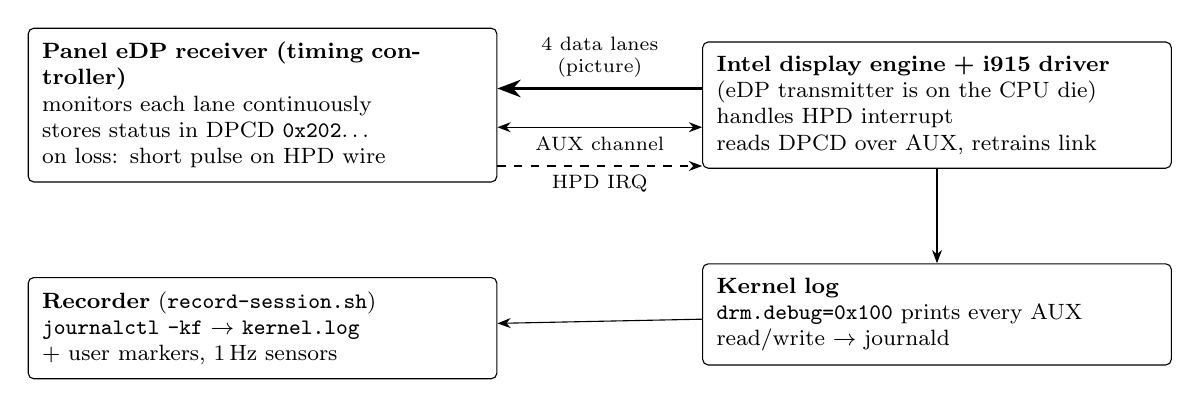
\begin{tikzpicture}[
  box/.style={draw,rounded corners=2pt,align=left,font=\footnotesize,inner sep=5pt,text width=5.6cm},
  lbl/.style={font=\scriptsize,align=center},
  >=Stealth]
\node[box] (panel) {\textbf{Panel eDP receiver (timing controller)}\\
  monitors each lane continuously\\ stores status in DPCD \reg{0x202}\ldots\\ on loss: short pulse on HPD wire};
\node[box,right=2.6cm of panel] (gpu) {\textbf{Intel display engine + i915 driver}\\
  (eDP transmitter is on the CPU die)\\ handles HPD interrupt\\ reads DPCD over AUX, retrains link};
\node[box,below=1.2cm of gpu] (log) {\textbf{Kernel log}\\ \reg{drm.debug=0x100} prints every AUX\\ read/write $\to$ journald};
\node[box,below=1.2cm of panel] (rec) {\textbf{Recorder} (\reg{record-session.sh})\\ \reg{journalctl -kf} $\to$ \reg{kernel.log}\\ + user markers, 1\,Hz sensors};
\draw[->,very thick] ([yshift=6pt]gpu.west) -- node[lbl,above]{4 data lanes\\(picture)} ([yshift=6pt]panel.east);
\draw[<->] ([yshift=-8pt]gpu.west) -- node[lbl,below]{AUX channel} ([yshift=-8pt]panel.east);
\draw[->,dashed] ([yshift=-22pt]panel.east) -- node[lbl,below]{HPD IRQ} ([yshift=-22pt]gpu.west);
\draw[->] (gpu) -- (log);
\draw[->] (log) -- (rec);
\end{tikzpicture}
\caption{The panel detects the loss and signals it. The Intel driver reads and logs the status. The recorder captures the log.}
\end{figure}

\noindent The read pattern \reg{0x200} $\to$ \reg{0x2005} $\to$ \reg{0x202} $\to$ \reg{0x200b} matches the driver servicing a
short-pulse HPD interrupt from the panel. This is inferred from the pattern: the DP debug category does not print the word ``HPD''
(the KMS category, \reg{drm.debug=0x106}, would).
The same register reads also occur during \emph{deliberate} link training (mode changes, display power-on, resume). Those
periods were identified by their timing and excluded.

%=====================================================================
\section{Why 240\,Hz fails and 60\,Hz does not}
%=====================================================================
The panel's supported eDP link rates (DPCD \reg{0x010}, 16-bit values in units of 200\,kHz) are 1.62, 2.16, 2.43, 2.7, 3.24, 4.32,
5.4 and 8.1\,Gbit/s per lane. The link-rate index the driver writes to \reg{0x115} during training shows:

\begin{center}
\begin{tabular}{@{}l c c@{}}
\toprule
Refresh rate & \reg{0x115} index & Per-lane rate\\
\midrule
240\,Hz & 7 & \textbf{8.1\,Gbit/s} (HBR3, panel maximum)\\
60\,Hz & 5 & 4.32\,Gbit/s\\
\bottomrule
\end{tabular}
\end{center}

\noindent At 240\,Hz each lane carries almost twice the data, so each bit lasts about 0.12\,ns instead of 0.23\,ns. A connection
with reduced signal integrity fails first at the higher rate.

%=====================================================================
\section{Causes ruled out}
%=====================================================================
\begin{itemize}
\item \textbf{Battery or voltage drop:} reproduced on AC power, battery voltage steady at 12.26--12.70\,V.
\item \textbf{Display engine starved of memory bandwidth by the RAM test:} i915 always logs a FIFO underrun error in that case. There were \textbf{zero}.
\item \textbf{Compositor page-flip errors} (logged by sway in the recorded tests as \reg{Atomic commit failed: Device or resource busy}): these occur in normal use without visible
artifacts. They are a side effect of the driver being busy, not the cause.
\item \textbf{Suspend/resume or display power cycling:} tested directly and did not reproduce it. The display restored correctly after every resume.
\item \textbf{GPU heat or GPU power alone:} 12 minutes at $\approx$\SI{88}{W} / \SI{76}{\celsius} (GPU only) produced no events.
\item \textbf{Panel Self Refresh (PSR) or variable refresh rate:} PSR was disabled by kernel argument (\reg{i915.enable\_psr=0}) and
VRR was off for all experiments.
\item \textbf{A specific distribution or desktop environment:} CachyOS and Fedora Workstation, and GNOME, Hyprland and sway, have been tried.
\end{itemize}

%=====================================================================
\section{Interpretation}
%=====================================================================
\begin{enumerate}
\item The physical eDP link loses lock. This is measured directly in the panel's status registers, and the single-lane failure
(\reg{17 77}) is characteristic of a signal-integrity problem in a cable or connector rather than software.
\item The trigger is CPU+RAM load combined with GPU load, at 240\,Hz. CPU package temperatures were similar with and without the
failure (77 vs.\ 80\,\si{\celsius}), so measured heat alone is a weak explanation.
\item \textbf{Leading hypothesis:} on Intel laptop CPUs the display engine and its eDP output circuitry are on the CPU die. Heavy core
and memory-controller activity causes large, fast current transients and switching noise in the CPU package and its voltage regulators,
right where the eDP signal starts. A healthy cable and connector have enough margin to tolerate this at 8.1\,Gbit/s. A
poorly seated, damaged or out-of-spec connection does not.
\item Once margin is lost, it stays lost while the load continues. The link flaps (lines), the driver retrains it (about 1\,s blackout), and the cycle repeats.
\end{enumerate}

%=====================================================================
\section{How to reproduce}
\label{sec:repro}
%=====================================================================
\subsection{Visual reproduction}
\begin{enumerate}
\item Set the internal panel to \textbf{2560$\times$1600 at 240\,Hz}.
\item Connect AC power.
\item Download OCCT from \url{https://www.ocbase.com/} and start it on the NVIDIA GPU:
\begin{lstlisting}[language=bash]
__NV_PRIME_RENDER_OFFLOAD=1 __GLX_VENDOR_LIBRARY_NAME=nvidia ./OCCT
\end{lstlisting}
\item Run a \textbf{combined CPU+RAM and GPU stress test} for at least 10 minutes: OCCT \emph{CPU+RAM}, \emph{3D Adaptive}
and \emph{VRAM} running together.
\item Expected result: thin lines and blackouts within about 2--5 minutes of adding the CPU+RAM load (1\,min\,50\,s in the controlled run).
\item Control: repeat at \textbf{60\,Hz}. Expected result: no artifacts.
\item Optional: while the fault is active, gently flex the lid or press along the bottom bezel near the hinges. A change in the
artifacts points to the cable or connector.
\end{enumerate}

\subsection{Reproduction with link-level evidence}
These steps work under any desktop environment. In the provided GNOME test account (Section~\ref{sec:testenv}) the preparation steps are already done.
\begin{enumerate}
\item Log in to the test account (or boot Linux from a live USB). Set the panel to 240\,Hz (GNOME: \emph{Settings $\to$ Displays $\to$ Refresh Rate}).
\item Enable DP debug logging:
\begin{lstlisting}[language=bash]
sudo sh -c 'echo 0x100 > /sys/module/drm/parameters/debug'
\end{lstlisting}
\item Start watching the panel's link status:
\begin{lstlisting}[language=bash]
journalctl -kf -o short-precise \
  | grep --line-buffered '0x00202 AUX' \
  | grep --line-buffered -v ') 77 77'
\end{lstlisting}
\item Leave the laptop idle for 5 minutes. Expected result: no output.
\item Start the combined CPU+RAM + GPU load. Expected result: lines such as
\begin{lstlisting}
... AUX A/DDI A/PHY A: 0x00202 AUX -> (ret=  6) 00 00 80 00 00 00
\end{lstlisting}
appear at the same moments as the artifacts.
\item Stop the load, switch to 60\,Hz (GNOME: \emph{Settings $\to$ Displays $\to$ Refresh Rate}), and repeat. Expected result: no output, apart from one \reg{11 11} read at the moment of the
mode switch (normal training).
\end{enumerate}
\noindent The complete automated procedure used for this report (recorder, marker tool, phase reminders) is in Appendix~\ref{app:scripts}.

%=====================================================================
\section{Test environment provided to technicians}
\label{sec:testenv}
%=====================================================================
\begin{itemize}
\item A dedicated \textbf{test user account} will be provided on the laptop. Its desktop environment is \textbf{GNOME} (Wayland).
\item Its \textbf{home folder contains the test cases}: the scripts in Appendix~\ref{app:scripts} and step-by-step instructions.
\item The recorded sessions in this report were made under sway. The scripts are desktop-independent: they detect GNOME, sway or
Hyprland and read the refresh rate through each desktop's own interface. The fault itself is in the eDP link and does not depend on the desktop.
\item On start, \reg{record-session.sh} checks that the account can read the kernel log and that DisplayPort debug lines are present,
and prints a warning if not.
\item Results of each run are saved in a timestamped folder (\reg{meta.txt}, \reg{kernel.log}, \reg{journal.log}, \reg{monitor.csv}), which can be sent back for comparison.
\end{itemize}

%=====================================================================
\section{Contact}
%=====================================================================
If you have any problems reproducing the fault, using the test account or reading the data, please feel free to email
\textbf{Yuechao Liu} at \href{mailto:yuechao.liu29@gmail.com}{\texttt{yuechao.liu29@gmail.com}}.

%=====================================================================
\section{Limitations}
%=====================================================================
\begin{itemize}
\item Decoding the DPCD bytes is our interpretation of the DisplayPort register layout. The kernel prints only the raw bytes.
\item Not every visible glitch produces a log entry. The driver reads status only when the panel raises an interrupt. In the
controlled run, flicker was visible from 21:08:41 to 21:21:13, while logged link losses span 21:09:26 to 21:18:57. The
match is therefore per episode, not per glitch.
\item Two reproductions on one machine on one day. Heat and electrical noise were not separated (suggested tests: CPU-only vs.\
RAM-only stress, a capped CPU power limit, and a start from cold).
\item Software cannot distinguish a faulty cable or connector from a marginal replacement panel.
\item No logs exist from before the panel replacement. The link to the repair rests on the user's report of when the problem started.
\item Under CPU load, the 1\,Hz sensor sampler slowed to one sample every 3--5\,s. The kernel log is unaffected.
\end{itemize}

%=====================================================================
\section{Conclusion and requested repair}
%=====================================================================
The internal eDP link between the mainboard and the replacement panel loses signal lock at its maximum link rate (8.1\,Gbit/s,
used for 240\,Hz) under sustained combined CPU and GPU load. The same load at 60\,Hz (4.32\,Gbit/s) is clean. This behaviour started after
the panel replacement. We request:
\begin{enumerate}
\item reseat or replace the \textbf{eDP display cable} and inspect both connectors (mainboard and panel side) for damage,
contamination or incomplete seating;
\item confirm the replacement panel matches the original part (installed: CMN \reg{0x1652}, 2560$\times$1600 at 240\,Hz);
\item verify the repair at \textbf{240\,Hz under at least 10 minutes of combined CPU+RAM and GPU stress}. Idle or 60\,Hz testing will not show the fault.
\end{enumerate}
Until then, running the panel at 60\,Hz avoids the problem.

\appendix
%=====================================================================
\section{Data files}
%=====================================================================
Available in the investigation folder \reg{screen-flicker-investigation/}:
\begin{center}
\small
\begin{tabularx}{\linewidth}{@{}l Y@{}}
\toprule
\reg{runs/2026-11-23\_20-43-06/} & controlled session: \reg{kernel.log} (DP debug), \reg{journal.log}, \reg{monitor.csv}, \reg{meta.txt}, \reg{ANALYSIS.md}\\
\reg{evidence/} & first reproduction (20:15 onward): kernel DP debug log, link-status reads, monitor CSV with markers\\
\reg{full-logs/} & complete journal of every boot since 21 Nov 2026 (compressed)\\
\reg{system-info/} & hardware list, versions, panel EDID (binary), driver parameters, sway outputs\\
\reg{repro/} & recorder, marker tool and test scripts\\
\bottomrule
\end{tabularx}
\end{center}
The full logs contain general system activity and are available on request.

%=====================================================================
\section{Scripts}
\label{app:scripts}
%=====================================================================
\subsection{\texttt{record-session.sh}: session recorder}
\lstinputlisting[language=bash]{../repro/record-session.sh}
\subsection{\texttt{mark.sh}: flicker and phase marker}
\lstinputlisting[language=bash]{../repro/mark.sh}
\subsection{\texttt{display-info.sh}: desktop detection (GNOME, sway, Hyprland)}
\lstinputlisting[language=bash]{../repro/display-info.sh}

\end{document}
